%%%%%%%%%%%%%%%%%%%%%%%%%%%%%%%%%%%%%%%%%%%%%%%%%%%%%%%%%%%%
%%% DOCUMENT PREAMBLE %%%
\documentclass[english, a4paper]{report}
\usepackage[T1]{fontenc}            % Riktig fontencoding
\usepackage[font=small, labelfont=bf]{caption} % Fin figur-undertekst
\usepackage{url}                    % Skrive url-er
\usepackage[english]{babel}         % Ordelingsregler, osv (velg språk her)
\usepackage[utf8]{inputenc}         % Riktig tegnsett
\usepackage{float}                  % Figurer dukker opp der du ber om
\usepackage{amsmath} 
\usepackage{graphicx}               % Inkludere bilder
\usepackage{subcaption}				% for subfigures environments
\usepackage[backend=biber, style=ieee, sortcites=true]{biblatex}
\usepackage{csquotes}
\graphicspath{{images/}}
%\usepackage{listings}               % programeringskode
%\usepackage{minted}                 % for coding
%\usepackage{xcolor}                 % for coding
% ---------------------------------------------------------

\addbibresource{../references.bib}

% kapittelinndeling
\renewcommand{\thepart}{\arabic{part})}
\renewcommand\thesection{\arabic{section}}
\renewcommand{\thesubsection}{\alph{subsection})} % Alph = ABC, alph = abc
\renewcommand{\thesubsubsection}{\roman{subsubsection})}

%---------------------------------------------------------
\pdfinfo{
%   /Title () 
	/Author (Henrik Løland Gjestang) 
	/Creator () 
	/Producer () 
	/Subject () 
	/Keywords () 
}
% ---------------------------------------------------------
%%% DOCUMENT PREAMBLE END%%%
%%%%%%%%%%%%%%%%%%%%%%%%%%%%%%%%%%%%%%%%%%%%%%%%%%%%%%%%%%%%


%-----------------------------------------------------------
% Forside
% ----------------------------------------------------------
\begin{document}
\begin{titlepage}
  \begin{center}

  \textsc{}\\[1.0cm]
  \textsc{\Large Master essay}\\[0.5cm]
  \rule{\linewidth}{0.5mm} \\[0.4cm]
  {\huge \bfseries A look on neural networks}\\[0.10cm]
  \rule{\linewidth}{0.5mm} \\[1.5cm]
  \textsc{}\\[7.0cm]

  \begin{minipage}{0.69\textwidth}
    \begin{center} \large
      Henrik Løland Gjestang\\ \url{henriklg@fys.uio.no} \\[0.8cm]
    \end{center}
  \end{minipage}
  \vfill

  % Dato nederst
  \large{Date: \today}
  \end{center}
\end{titlepage}


% ----------------------------------------------------------
% Abstract, table of contents, List of figures/tables
% ----------------------------------------------------------
\tableofcontents
\newpage
% ----------------------------------------------------------




%%%%%%%%%%%%%%%%%%%%%%%%%%%%%%%%%%%%%%%%%%%%%%%%%%%%%%%%%%%%
\section{Introduction}
%-----------------------------------------------------------
%Explain the aims and rationale for the physics case and what you have done. At the end of the introduction you should give a brief summary of the structure of the report. Motivate the reader and give overarching ideas. Describe what has been done and the structure of the report (how is it organized).

In this project, we aim to design and develop a system for analyzing medical videos from a camera pill, as seen in figure \ref{fig:pill-cam}. The pill is swallowed and records video of the entire digestive system and stores it on a onboard chip - the goal is to be able to detect different irregularities in the patients digestive system, like a colon polyp, Chron's disease, Colorectal cancer, etc. By using video object tracking, object detection, machine learning or other relevant tools or mechanisms.

Neural networks models that I would like to explore further for this purpose are Convolutional neural networks (CNN), Recurrent neural networks (RNN), Capsule neural networks, Long Short-Term memory networks and more.

The main idea is to go beyond image-based methods and also exploit the time factor of the data. 
The videos we will be using for this is delivered by Bærum Hospital, and is carefully labeled by professionals for use as training data for the neural networks. For simplicity, much or all of the training data is from regular "bottom-up" colonoscopy. 

\begin{figure}[H]
  \begin{center}
    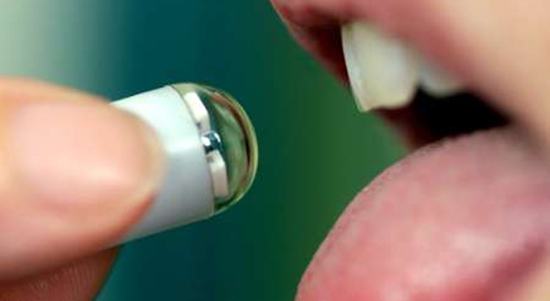
\includegraphics[width=\linewidth]{pill-cam.jpg}
    \caption{Illustration of how such a camera pill could look like.\autocite{PillCamCamera}}
    \label{fig:pill-cam}
  \end{center}
\end{figure}

Colorectal cancer (CRC) is the third most common cause of cancer mortality for both men and women \autocite{CancerStatistics10}, and it is a condition where early detection is of clear value for the ultimate survival of the patient. As statistics show that 15\% of male and female above 50 years are at risk (SOURCE), the procedure is recommended on a regular basis (every 3-5 years) for the population over 50, and from an earlier age for high-risk groups. Colonoscopy is a demanding procedure requiring an significant amount of time by specialized physicians, in addition to the discomfort and risks inherent in the procedure. Thus, traditional methods based on colonoscopy are not cost-effective for population-based screening purposes, so only about 2-3\% of the target population is reached at present. Moreover, the cost of a population screening program is prohibitively expensive. In the US, the colonoscopy is the most expensive cancer screening process with annual costs of \$10 billion dollars (\$1100 per person) (SOURCE). In Norway, we have similar costs of around \$1000 per person, with a time consumption of about 1 doctor-hour and 2 nurse-hours, per examination. By researching an automatic system for a camera pill, the aim is to greatly increase the number of patients that can be examined, i.e., making the public health care system more scalable and cost effective, while at the same time reducing the need for intrusive procedures like "bottom-up" examinations like colonoscopy.




%%%%%%%%%%%%%%%%%%%%%%%%%%%%%%%%%%%%%%%%%%%%%%%%%%%%%%%%%%%%
\section{Wireless Capsule Endoscopy}
%-----------------------------------------------------------
%general info about WCE, some history etc
The basic technology behind the modern endoscope was developed in the early 1950s by English physicist Harold Hopkins and his student Narinder Kapany which let light travel through flexible pieces of glass - now known as optical fibers. \autocite{NewMethod54}

Before the year 2000 the only option you had to visualize the foodpipe, stomach, duodenum, colon and terminal ileum (see figure \ref{fig:digestive_system} for details) was to use a fibre-optic endoscope, which is a tool with a relatively wide cable that is pushed into the bowel with as much as 50 000 optic fibers (as seen on figure \ref{fig:fibre-optic-endoscopy}). These cables have to carry fibre optic bundles, water pipes, operations channel and control cables. Although these cables can be quite flexible there is a limit for how far they can advance into the small bowel. This method cause pain and discomfort for the pasient, and there was a clinical need for an improved methods.

\begin{figure}
  \begin{center}
    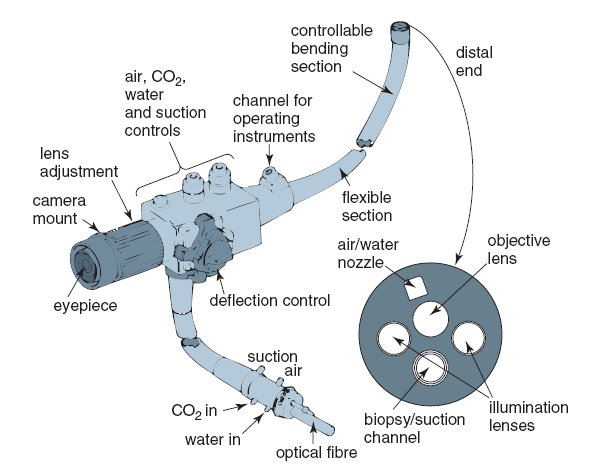
\includegraphics[width=0.7\textwidth]{fibre-optic-endoscopy}
    \caption{Image of a fibre optic endoscope with explanation of different parts of the tool. \autocite{MedicalPhysics}}
    \label{fig:fibre-optic-endoscopy}
  \end{center}
\end{figure}

\begin{figure}
  \begin{center}
    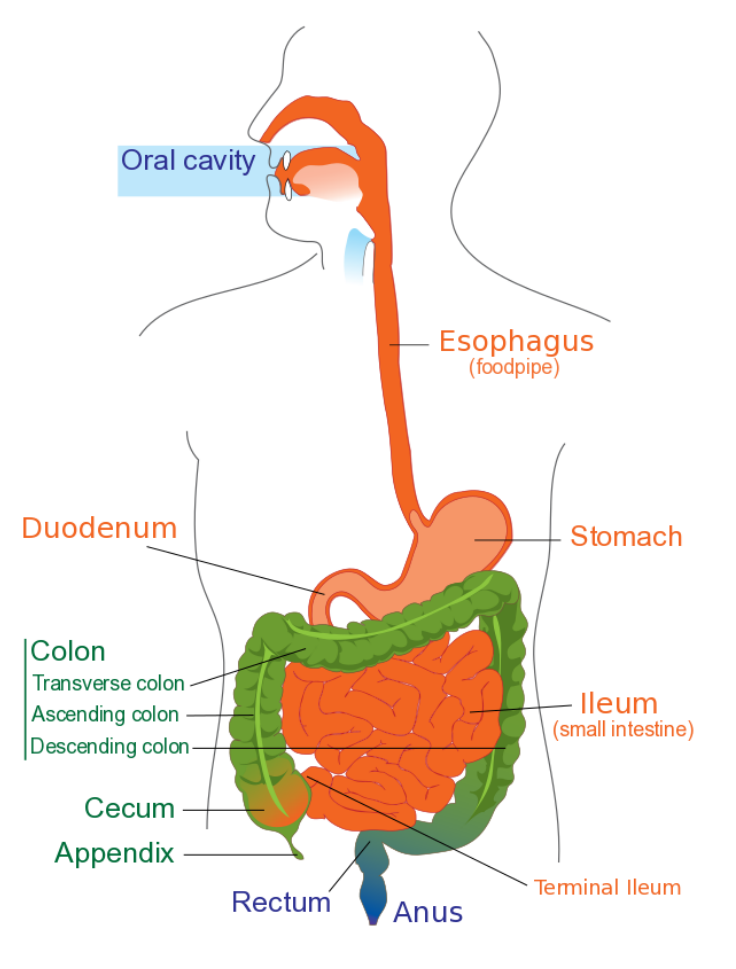
\includegraphics[width=0.7\textwidth]{digestive-system}
    \caption{An overview of the terms used to describe the digestive system. \cite{DigestiveSystem} }
    \label{fig:digestive_system}
  \end{center}
\end{figure}

That is why in the year 2000 Iddal et al.\autocite{WirelessCapsule00} developed a new type of videotelemetry capsule endoscope that was swallowable. It could travel through the entire digestive system because it had no external wires, fibre-optic bundles or cables of any sort. The capsule travels by peristalsis\footnote{Peristalsis is a radially symmetrical contraction and relaxation of muscles that propagates in a wave down a tube, in an anterograde direction.} through the gastroitestinal tract, which takes from 10 hours to 48 hours, and transmit images on a regular interval to recievers attached around the outside of the pasients stomach for as long as the battery allows, usually in the range 6-8 hours. Two example images taken by WCE are presented in Figure \ref{fig:pillcam_examples}. By triangulating the signal strength and the location of the receivers taped on the body it is possible to calculate the position of the capsule.

\begin{figure}%
  \centering
  \begin{subfigure}[b]{0.4\linewidth}%
    \centering
    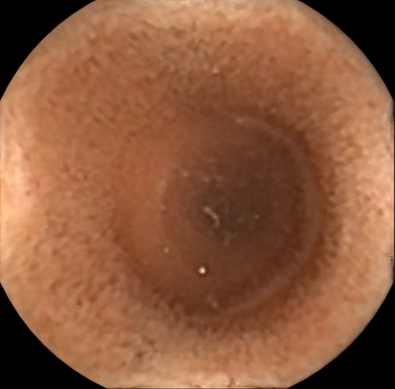
\includegraphics[width=\linewidth]{pillcam_small_intestine}%
    \caption{Small Intestine \cite{SmallIntestine13} }%
    \label{fig:pillcam_small_intestine}%
  \end{subfigure}%
  \quad
  \begin{subfigure}[b]{0.4\linewidth}%
    \centering
    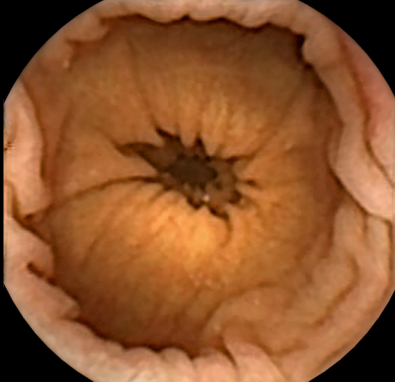
\includegraphics[width=\linewidth]{pillcam_colon}%
    \caption{Colon \cite{Colon13} }%
    \label{fig:pillcam_colon}%
  \end{subfigure}%
  \caption{Images taken with WCE.}%
  \label{fig:pillcam_examples}%
\end{figure}%


%%%%%%%%%%%%%%%%%%%%%%%%%%%%%%%%%%%%%%%%%%%%%%%%%%%%%%%%%%%%
\section{Spotting irregulartities in the digestive system}
%-----------------------------------------------------------
%what to look for when analyzing videos from the digestive system

To detect irregularities in the digestive system (figure \ref{fig:digestive_system} is a difficult task and time-consuming. To classify irregularities correctly and precisely require expert knowledge. Furtunately we have access to data which already has been labeled by trained proffesionals that we will use in this project. However I feel that some very basic knowledge in the subject will come in handy.

The most common way of screening pasients is with a endoscope. When this tool is used by a trained proffessional some of the irregularities that can be spotted are; \textit{Colon polyp}, \textit{Colorectal Cancer}, \textit{Ulcerative Colitis}, \textit{Crohn's Disease}, \textit{Familial adenomatous polypsis}, \textit{Diverticulosis} and \textit{Diverticula Bleeding}. 

These diseases have varying patterns and while some can be easy to split apart, some are more similar in pattern. While for an untrained eye it can be easy to spot that something is wrong it is very difficult to describe with words what that might be, or even harder to write a program to detect the correct characteristic features of the disease. This is why we rely on having good labeled data, and a good amount of it, for this project to work. I also imagine having to select one or two diseases to focus on. Preferebly two irregularities that both have different characteristics and lots of labele dtraining data.






%%%%%%%%%%%%%%%%%%%%%%%%%%%%%%%%%%%%%%%%%%%%%%%%%%%%%%%%%%%%
\section{Neural network models}
%-----------------------------------------------------------
%explain the different neural networks I'd like to test out on the video
As apposed to using regular optic-fibre endoscopy, it can be difficult to know the location and orientation of the capsule when it is traveling through the digestive system. In a paper by \citeauthor*{ClassifyingDigestive15} \cite{ClassifyingDigestive15} it is shown that by using Deep Convolutional Networks (DCNN) it is possible to classify the digestive organs in wireless capsule endoscopy with about 95\% classification accuracy on average. 

The DCNN-based WCE digestive organ classifiaction system is constructed of three stages of convolution, pooling and two fully-connected layers. This is illustrated in figure 3 in the paper. \cite{ClassifyingDigestive15}






\subsubsection{Convolution layer}
% ----------------------------------------------------------
The first step in a convolutional neural network is to extract features from the input image. This is done to preserve the relationship between pixels by learning image features using filters, or \textit{kernels}. As a result, the network learn filters that activate when it detects some specific patterns or features.

The convolution of \textit{f} and \textit{g} is written as $f*g$, and is defined as the integral of the product of the two functions after one (usually the filter) is reversed and shifted.

\begin{equation}
  (f*g)(t) = \int_{-\infty}^{\infty} f(\tau) g(t-\tau) d\tau
  \label{convolution_func}
\end{equation}


% ----------------------------------------------------------
\subsubsection{Non Linearity (ReLU)}
% ----------------------------------------------------------
Rectified Linear unit function, known as simply ReLU, is an activation function represented by equation (\ref{relu_func}). It sets all negative numbers to zero, by discarding them from the activation map entirely. In this way, ReLU increases the nonlinear properties of the decision function and thus of the overall network without affecting the receptive fields of the convolution layer.

\begin{equation}
    ReLU(x) = max(0, x)
    \label{relu_func}
\end{equation}


% ----------------------------------------------------------
\subsubsection{Pooling layer}
% ----------------------------------------------------------
Pooling layers are applied to reduce the number of parameters when the images are considerably large. Spatial pooling, or merely downsampling, reduces the dimensionality of each image but it keeps the important information. The most used downsampling is max pooling. It extracts the largest element from the rectified feature map and thus reduces computational complexity of the algorithm. In addition average pooling is also frequently used, this method computes the average value of the input map. The input-output model is denoted as:

\begin{equation}
  y_i = f(pool(x_i))
  \label{pool_func}
\end{equation}


% ----------------------------------------------------------
\subsubsection{Fully-connected layer}
% ----------------------------------------------------------
In a FC-layer every neuron in one layer is connected to every neuron in the previous layer. It is here the high-level reasoning is done. The activation function in the neurons is a \textit{sigmoid} or \textit{tanh} function.

\begin{equation}
  f(z) = \frac{1}{1+exp(-z)} \quad \text{or} \quad f(z) = tanh(z) = \frac{e^{z} - e^{-z}}{e^{z} + e^{-z}}
\end{equation}

At the end of FC-layer we have an activation function such as softmax (equation \ref{softmax}) to calculate probability of the predicted classes.


% ----------------------------------------------------------
\subsubsection{Feed Forward}
% ----------------------------------------------------------
In the feed forward algorithm input image will be processed through all the layers in the neural network. The first layer will be a convolution layer, containing $K$ filters $F_i^1$, $i= 1, ..., K$, of size $k \times k$ and a bias $b^1$. The image will be convoluted with each filter, and the bias is added. 

\begin{equation}
    \hat{z}_i^l = I * \hat{F}_i^l + b^l, 
\end{equation}

where $*$ (asterisk) is the convolution operator in equation \ref{convolution_func}. The final output of each convolutional layer $l$ is $a^l$,

\begin{equation}
    \hat{a}_i^l = f(z_i^l), 
\end{equation}

where $f$ represents the ReLU activation function. After going through the convolution layer, the next layer could be a pooling layer, which will reduce the spatial dimensionality either by using the max value or the average value.
Before getting our final output $\hat{y}$, we need to collect the outputs from all the filters, which will be an input to a fully connected layer. 
The fully connected layer use the softmax activation function to classify the input image, much like a neural network would. The softmax function is an accepted standard probability function for a multiclass classifier \cite{NotesBackpropagation16}. The total sum of the probabilities will always add up to 1 when using softmax. 

\begin{equation}
  \sigma(z)_j = \frac{e^{z_j}}{\sum_{k=1}^{K} e^{z_k}} \quad \text{for } j = 1, ..., K.
  \label{softmax}
\end{equation}

To calculate the error of the forward propegation it is common to use cross-entropy error function.

\begin{equation}
  C(\hat{y}) = - \sum_{i=1}^N t_i log(y_i)
  \label{loss}
\end{equation}


% ----------------------------------------------------------
\subsubsection{Backpropagation}
% ----------------------------------------------------------
Starting from the last layer $L$, we calculate the derivative of the loss function (function \ref{loss}) with regards to the activation function in order to update the weights. Computing the gradient of the loss function yields

\begin{equation}
  \frac{\partial C}{\partial y_i} = - \frac{t_i}{y_i}
\end{equation}

We also require the gradient of the output of the final layer $y_i$ with regards to the input $z_k^L$ of the activation function (equation \ref{softmax})

\begin{equation}
  \frac{\partial y_i}{\partial z_k^L} = 
  \begin{cases}
      y_i(1 - y_i), & i = k\\
      -y_iy_k, & i \ne k
  \end{cases}
\end{equation}

Now with regards to $z_i^L$

\begin{equation}
  \begin{aligned}
  \frac{\partial C}{\partial z_i^L} &= \sum_k^N \frac{\partial C}{\partial y_k}\frac{\partial y_k}{\partial z_i^L} \\
  &= \frac{\partial C}{\partial y_i}\frac{\partial y_i}{\partial z_i^L} - \sum_k^N \frac{\partial C}{\partial y_k}\frac{\partial y_k}{\partial z_i^L} \\
  &= -t_i(1 - y_i) + \sum_{k \ne i}t_ky_i \\
  &= y_i - t_i
  \end{aligned}
\end{equation}

And finally with regards to the weights

\begin{equation}
   \frac{\partial C}{\partial w_ij^L} = (y_i - t_i)a_j^{L-1}
\end{equation}

where $\hat{a}_{j}^{L-1}$ is the vectorized output from the previous layer. From here, we will propagate the error throughout the layers. The error with regards to the input $a_i^L$ to the fully connected layer is:

\begin{equation}
  \delta^{L-1} = \frac{\partial C}{\partial a_i^L} = \sum_i^N (y_i - t_i)w_{ji}^{L}
  \label{back_error}
\end{equation}

Thus the error is propagated backwards through each layer. If max pooling was used in a pooling layer, the error will only be propagated to the input that had the highest value in the forward pass. The other values will be set to zero. If average pooling was used, the error is averaged in the backwards pass.
In equation \ref{back_error} $a^l$ is the output of a convolutional layer $l$. Since a convolutional layer is always preceded and followed by a activation layer, the input to layer $l$ is $a^{l-1} = \sigma(z^l)$. Now consider the error with regards to $z^l$

\begin{equation}
  \begin{aligned}
  \delta_{ij}^l &= \frac{\partial C}{\partial z_{ij}^l} \\
  &= \sum_i' \sum_j' \frac{\partial C}{\partial z_{i'j'}^{l+1}}\frac{\partial z_{i'j'}}{\partial z_{ij}^l} \\
  &= \sum_{i'} \sum_{j'}\delta_{i'j'}^{l+1} \frac{\partial (\hat{W}\sigma(z^l) + b^{l+1})}{\partial z_{ij}^l} \\
  &= \delta^{l+1} * ROT180(w^{l+1})\sigma'(z^l)
  \end{aligned}
\end{equation}

Having found the error, the gradient of the cost function with regards to the weights is

\begin{equation}
  \frac{\partial C}{\partial w_{ij}^l} = \delta_{ij}^l * \sigma{ROT180(z_{ij}^{l-1})}
\end{equation}





\subsection{Object trackng}
%-----------------------------------------------------------
Object tracking is one of the harder problem to overcome in computer vision and is key to achieving good results in endoscopic video analysis. Tracking algorithms are developed to determine the movement of the object or objects in each video frame. The algorithm has to take into account the dynamic environment such as differences in lightning, occlusions and scaling changes. Also the absence of any prior knowledge to the object and its position further increase the complexity of the problem.

\begin{figure}[H]
  \begin{center}
    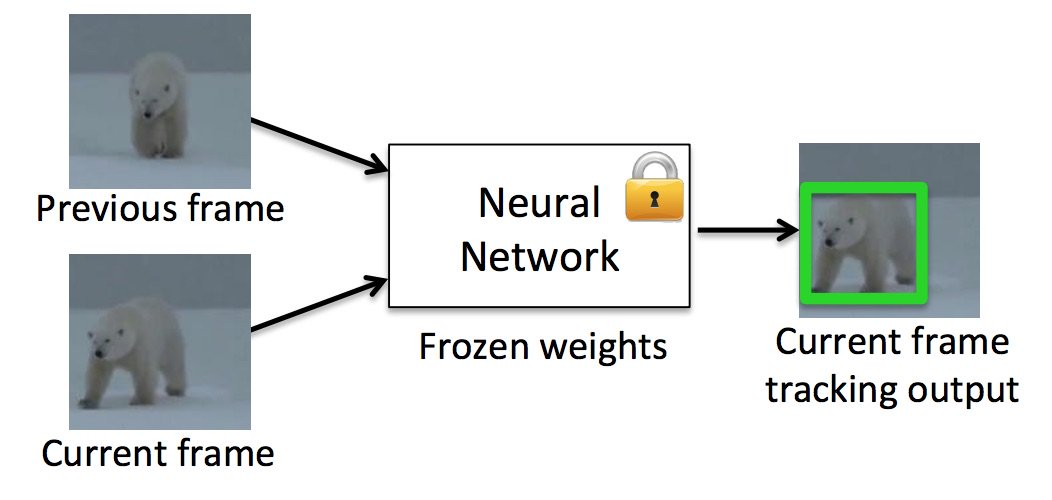
\includegraphics[width=\textwidth]{object-tracking.jpg}
    \caption{Illustration of how object in two frames is tracked with a bounding box. \cite{GOTURNDeep} }
    \label{fig:object-tracking}
  \end{center}
\end{figure}




%%%%%%%%%%%%%%%%%%%%%%%%%%%%%%%%%%%%%%%%%%%%%%%%%%%%%%%%%%%%
\section{Results and discussion}
%-----------------------------------------------------------
Present the results. Give critical discussion of your work and place it in the correct context. Try to relate your work to other calculations/studies. The reader should be able to reproduce your calculations if they wanted to. Remember to explain all input variables. Make sure figures and tables contain enough information in their captions/labels/axis so that the reader can gain a first impression of your work.





\newpage
\printbibliography

\end{document}